\documentclass{article}
\usepackage{amsfonts}
\usepackage{graphicx}
\usepackage[margin=1in]{geometry}
\usepackage{bm}
\title{Notes on applying gene set enrichment to microbiome analyses}
\author{Quang Nguyen}
\begin{document}
\maketitle

\section{Gene set analysis in the context of the microbiome}
\section{Methods involving trees}
\section{Some hypotheticals and further considerations}
\subsection{Approach 1: Taxonomic aggregation using isometric log-ratio transformations}
\subsubsection{Statistical interpretation of taxonomic aggregation using elementwise summations}

\indent Most microbiome studies have performed taxonomic aggregation through element-wise summation of the count vectors for all taxa assigned to the taxonomic rank of interest. Prior to statistical analysis, these aggregated counts are then usually converted to relative abundances by dividing by the total counts per sample, effectively normalizing for differences in library size. This compositional closure operation is unavoidable as "size-factors" can't be estimated from most microbiome data sets due to a lack of "consistent features" similar to that of housekeeping genes or UMIs in RNA-seq type studies. As such, we can define the classical taxonomic aggregation processs as simply the element-wise summation of compositional parts (or proportions). Let $P_{i}$ be the relative abundance of higher taxonomic rank (HTR) P (indexed by $\mathbb{P}$) in sample $i$ with raw counts $x_{ij}$ where $j$ is the column index of the lower taxonomic rank (LTR), as such:
$$P_{i} =\frac{\sum_{j \in \mathbb{P}} x_{ij}}{\sum x_{ij}} = \sum_{j \in \mathbb{P}} \frac{x_{ij}}{\sum x_{ij}} = \sum_{j \in \mathbb{P}} c_{ij}$$

\noindent Downstream analyses follow principles of compositional data analysis \cite{gloor2017}, which usually involves analyzing ratios of aggregated LTRs. These log-ratio analyses with aggregated compositions are termed "groups of amalgamated parts" analysis in the CoDA literature \cite{egozcue2005}. 

\noindent However, as Egozcue et al. \cite{egozcue2005} pointed out, amalgamated compositions are not equivalent to their original form. For example, take a simple composition of 3 parts $x = [x_1, x_2, x_3]$ and the aggregated composition $y = [x_1 + x_2, x_3]$ (with $n$ samples). The center \cite{aitchison} of the initial composition is 
$$cen(x) = \mathcal{C}\left[ \prod^n x_1, \prod^n x_2, \prod^n x_3 \right]$$ 
while the center of the aggregated composition is 
$$cen(y) = \mathcal{C}\left[ \prod^n (x_1 + x_2), \prod^n x_3 \right]$$
These two centers are very different, which also then translates to differences in the inter-sample Aichison distance after transformation. This invariant in inter-sample distance after aggregation means that aggregation distorts the original composition, and can attenuate differences in samples even if they're just noise (Figure 1) \cite{egozcue2005}. Even though other studies contend that aggregation is still viable \cite{greenacre2020}, we contend that this distortion effect is significant in microbiome analyses, which relies a lot on distance based methods.  

\begin{figure}[!htb]
    \centering
    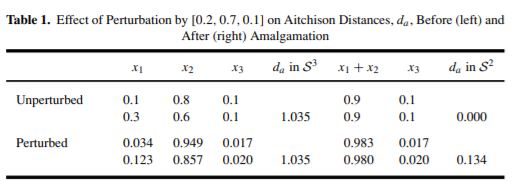
\includegraphics[scale=1.0]{ezogue_tab1.png}
    \caption{Table from Egozcue et al. demonstrating alterations of sample distances after aggregation}
    \label{fig:ezogue_tab1}
\end{figure}

\subsubsection{Competitive gene set testing using isometric log-ratios}
In order to solve this amalgamation issue, Egozcue et al. proposed the isometric log ratio (ilr) transformation \cite{egozcue2003}. In essence, ilr transform is a projection of the composition from the Aichison space to an orthonormal basis that exists in the simplex. This allows for the usage of standard statistical techniques as the composition is "opened" as well as being geometrically coherent compared to other flavors of log-ratio transforms. Conveniently, a sequential binary partition (SBP - which is a tree) is a valid orthonormal basis where the composition can be projected onto \cite{egozcue2003}. The transformed ilr coordinates are the tree nodes, which represent "balances" between two sides of the node. 
\begin{figure}[!htb]
    \centering
    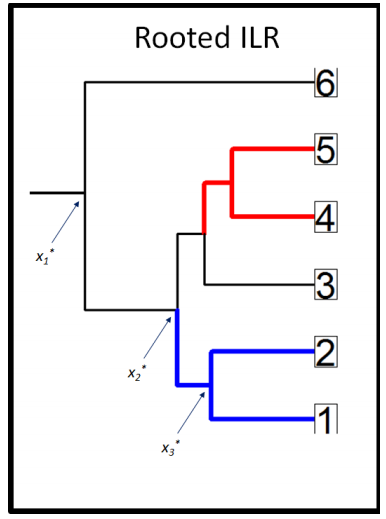
\includegraphics[scale = 0.5]{phylogeny_demonstration.png}
    \caption{A sample SBP in tree form which is also the phylogenetic tree}
    \label{fig:phylogeny_demonstration}
\end{figure}
In figure 2 is a toy example the ilr transformation on top of a phylogenetic tree. Each node $x_1^*, x_2^*, x_3^*$ represents the transformed ilr coordinates. The ilr transformation is defined as follows:
$$x_i^* = \sqrt{\frac{l}{r + l}} \log \left(\frac{g(\bm{x}_{j \in \bm{L}})}{g(\bm{x}_{j \in \bm{R}})}\right)$$
where $\bm{x}$ is the compositional vector, $g()$ is the geometric mean, $\bm{L}$ is the set of size $l$ of all parts on the left side of the node, and $\bm R$ is the set of size $r$ of all parts on the left side of the node. Note that $\bm L$ and $\bm R$ are non-overlapping sets. For the example in Figure 2, we have: 
$$x_2^* = \sqrt{\frac{2}{2 + 3}} \log \left( \frac{(x_1x_2)^{1/2}}{(x_3x_4x_5)^{1/3}}\right)$$
The ilr coordinate can be interpreted as the overall relative contribution of variables in $\bm L$ to the composition of $\bm L \cup \bm R$ weighted by the sizes of $\bm L$ and $\bm R$. This concept of balances have gained recent attention by the microbiome field, targeting transformations and dimension reduction along the phylogenetic tree \cite{washburne2017a, silverman2017a}. The ilr transformation 

\noindent Since the analysis of compositional data involves ratios of variables instead of individual factors, CoDA lends itself naturally to the gene set testing, specifically competitive gene set testing. 

\newpage
\bibliography{tax_agg}{}
\bibliographystyle{plain}
\end{document}
\end{document}